%---------------------------------------------
%        Scientific Report LaTeX Template
%             tex file
%            by Jac Thomas
%              16/01/2021
%         Jac.Thomas2@liverpool.ac.uk
%---------------------------------------------

% tells latex what kind of document this is, and optionally what size font.
\documentclass[11pt]{article}

% tells latex to load everything from preamble.sty in right here.
\usepackage{preamble}

% starts the document
\begin{document}

% prints out the document info (i.e. title, author, date) here
\maketitle

% prints out a table of contents, using the sections and page numbers.
\tableofcontents

% forces latex to start a new page, i.e. not just put the introduction
% section on the same page as the table of contents. if you wanted, you
% could put a \newpage command between \maketitle and \tableofcontents,
% so the title stuff and table of contents appear on separate pages.
\newpage

% this is how you start a new section.
\section{Examples}

\textbf{NB:} The PDF document and .tex file need to be read together. The best way to do this is have them open side-by-side in Overleaf. If you are completely new to \LaTeX, it is crucial that you read the latex\_tutorial.txt file before looking at this.

This is where you put your text, i.e. paragraph text. \textbf{This is how you write in bold,} and \textit{this is how you write in italics.} In this document I've included some sections and subsections, so delete/change them as necessary. This introduction contains some info and tips in subsections; after this introduction is just dummy text, i.e. text that is there just to show you what the document will look like with text in it. The dummy text was generated at \url{https://www.blindtextgenerator.com/}.

Notice that the start of the first paragraph in each section (or subsection) is not indented, but that all subsequent paragraphs in that section are indented. Though \LaTeX mostly ignores whitespace in your .tex file, when you hit enter and start a newline in your .tex file (see the line numbering on the left of the .tex file), \LaTeX will start a new paragraph. 

\subsection{Citations}

Here is a sentence with a single citation in brackets \parencite{Chan2015}. Here is a sentence with more than one citation in brackets \parencite{hfd2020,Clark2018}. In this sentence I write the author and then the year: \cite{wade2004}. Here are some other citations - note that I haven't cited everything in the .bib file in this document, so not everything in the .bib file will appear in the bibliography \parencite{stanphil,methmat2004,popprojections}. Only the items specified in the citations will appear in the bibliography.

\subsection{Equations}

Arguably the main strength of \LaTeX is how it handles mathematical expressions. Here is an example equation.

\begin{equation}
    P(x) = \frac{1}{\sigma \sqrt{2\pi}}e^{-(x_i -\mu)^2 / 2\sigma^2}.
\end{equation}

When you start an equation, you go into math mode. In math mode, there are a bunch more commands that you can use, to make mathematical expressions. For example, \textbackslash frac\{\}\{\} enables you to make a fraction, with the numerator in the first set of curly braces and the denominator in the second set. Equation (1) also includes the \textbackslash sqrt\{\} command: anything you write inside the curly braces will appear under a square root sign. Math mode also styles letters differently: compare $x$ (math mode) and x (text mode). Another thing which you will probably use frequently in math mode is Greek letters, which you get by writing a backslash and then the name of the Greek letter you want. The last important point is subscripts and superscripts: subscripts are made by writing an underscore (\_) like in $x_i$, and superscripts are made by writing a caret (\^{}) like in $x^2$. You can combine them like this $x_i^2$, and if your subscript or superscript is longer than a single character, you can just enclose it in curly braces: $x_{i+1}^{-1/3}$.

As you have probably noticed, we can also use math mode inside of paragraphs, i.e. not just in a separate equation. The way we do this is by enclosing the mathematical expression in a pair of dollar signs: \$x\^{}2\$. This is known as in-line math mode.

Equations are numbered by default, meaning that a number in brackets appears at the right-hand side of the equation in the PDF. To turn off automatic numbering of an equation, make this environment instead: \textbackslash begin\{equation*\} \textbackslash end\{equation*\}. If you want to write out a derivation down the page, you can use the align environment in the same way as the equation environment, and align equals signs on consecutive lines by putting the ampersand symbol (\&) before each equal sign. Here is an example, with automatic numbering turned off.

\begin{align*}
    y &= (x+4)^2 \\
    &= (x+4)(x+4) \\
    &= x^2 + 8x + 16.
\end{align*}

\subsection{Tables}

To make a table, there are a couple of things you should do. Firstly, you create a table environment, which will contain the table itself, as well as other things such as its title, its label (something you can use to refer to the table elsewhere in the document), and whether the table is centered. Then within the table environment, you create the tabular environment, which contains the actual rows and columns of the table. Here is an example table.

\begin{table}[h]
    \caption{Data table} % the title of the table
    \label{table:table1}% is used to refer this table in the text
    \centering % used to center the table
    \begin{tabular}{|c|c|c|p{5cm}|} % 3 centered columns then 1 fixed width column
        \hline                       %inserts a horizontal line
        Case & Method\#1 & Method\#2 & Method\#3 \\  % heading
        \hline                  % inserts single horizontal line
        1 & 50 & 837 & 48 \\ % info for each column on the first row, separated by & symbols
        \hline                  % inserts a single horizontal line
        2 & 47 & 877 & 230  \\
        \hline
        3 & 31 & 25  & 415  \\
        \hline
        4 & 35 & 144 & She had a last view back on the skyline of her hometown Bookmarksgrove, the headline of Alphabet Village and the subline of her own road, the Line Lane \\
        \hline
        5 & 45 & 300 & 485 \\
        \hline 
    \end{tabular}
\end{table}

As you can see, it begins with starting the table environment, along with the optional [h] command to tell \LaTeX to put the table `here,' i.e. as soon as possible after the sentence ``Here is an example table.'' We then specify the caption, give it a label, and make sure it's centered. Then we actually start making the table itself, with the tabular environment. Note that when we begin the tabular environment, we also need to specify the structure of the table in curly braces, using a combination of letters and symbols. Our specification is: \{|c|c|c|p\{5cm\}|\}. This means that we want 3 columns in which the text is centered, and then a fourth column in which the text is left-aligned, and which has a fixed width of 5cm. This prevents the text from spilling over the side of the page. The bars (|) tell \LaTeX that we want the columns to have vertical lines as borders, all the way down the rows. After beginning the tabular environment and specifying the column structure, you can start adding rows, separated by horizontal lines if you want. For each row, you must give as many elements as there are columns, and elements are separated using the ampersand symbol \&. For example, the first row in Table \ref{table:table1} after the heading is: 1 \& 50 \& 837 \& 48 \textbackslash \textbackslash. Because I specified that there should be 4 columns, I need to have 4 entries, separated by ampersands. The double backslash at the end tells \LaTeX to start a new line.

\subsection{Graphics}

It is straightforward to include graphics in \LaTeX -- you just need to make sure that your graphic (usually a .png file) is in the same folder as your main.tex file. To insert a graphic, it's usually best to do so within a `figure' environment (this is similar to how we put the tabular environment within the table environment). The figure environment automatically centers the graphic, and enables us to include a title, notes, and a label. The instruction to include a particular graphic is given by the \textbackslash includegraphics{} command, with the file name of the graphic in the curly braces. An important optional argument is [scale=0.5], which in this case scales the graphic to half of its original size. I usually have no idea how big my graphics ``really'' are, so I usually just keep changing this number and recompiling until it looks decent. Everything in Figure \ref{fig:prop_ev_marr} below the figure title and above `Notes' is just a picture, i.e. you can't edit the text on the graph. It is actually possible to produce figures from scratch in \LaTeX, but I don't know about such things.

\begin{figure}
    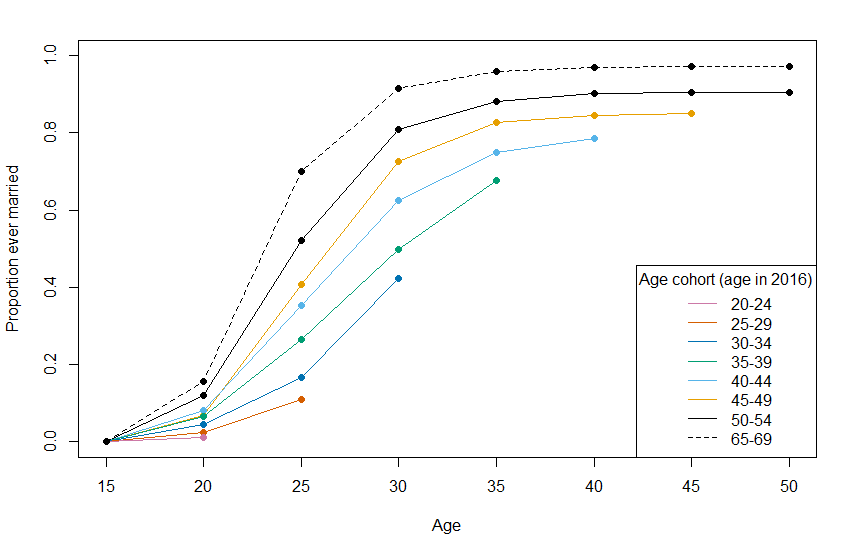
\includegraphics[scale=0.5]{prop_ev_marr.png}
    \caption{Proportion of Taiwanese women ever married by different ages, by age cohort in 2016.}
    \floatfoot{
        \noindent \textbf{Notes:} Data for this plot are from a sample survey, and are therefore not necessarily representative of the entire population. N=16,669.\\~\\
        \textbf{Source}: Women's Marriage, Employment and Fertility Survey (WMFES) 2016. Own calculations. Data available via application from the Survey Research Data Archive, Academia Sinica: \url{https://srda.sinica.edu.tw/index_en.php}.}
    \label{fig:prop_ev_marr}
\end{figure}

I've also included another figure, which is just a screenshot of this folder open in Overleaf. I just include it so that you know what you should be looking at when you're reading the PDF.

\begin{figure}
    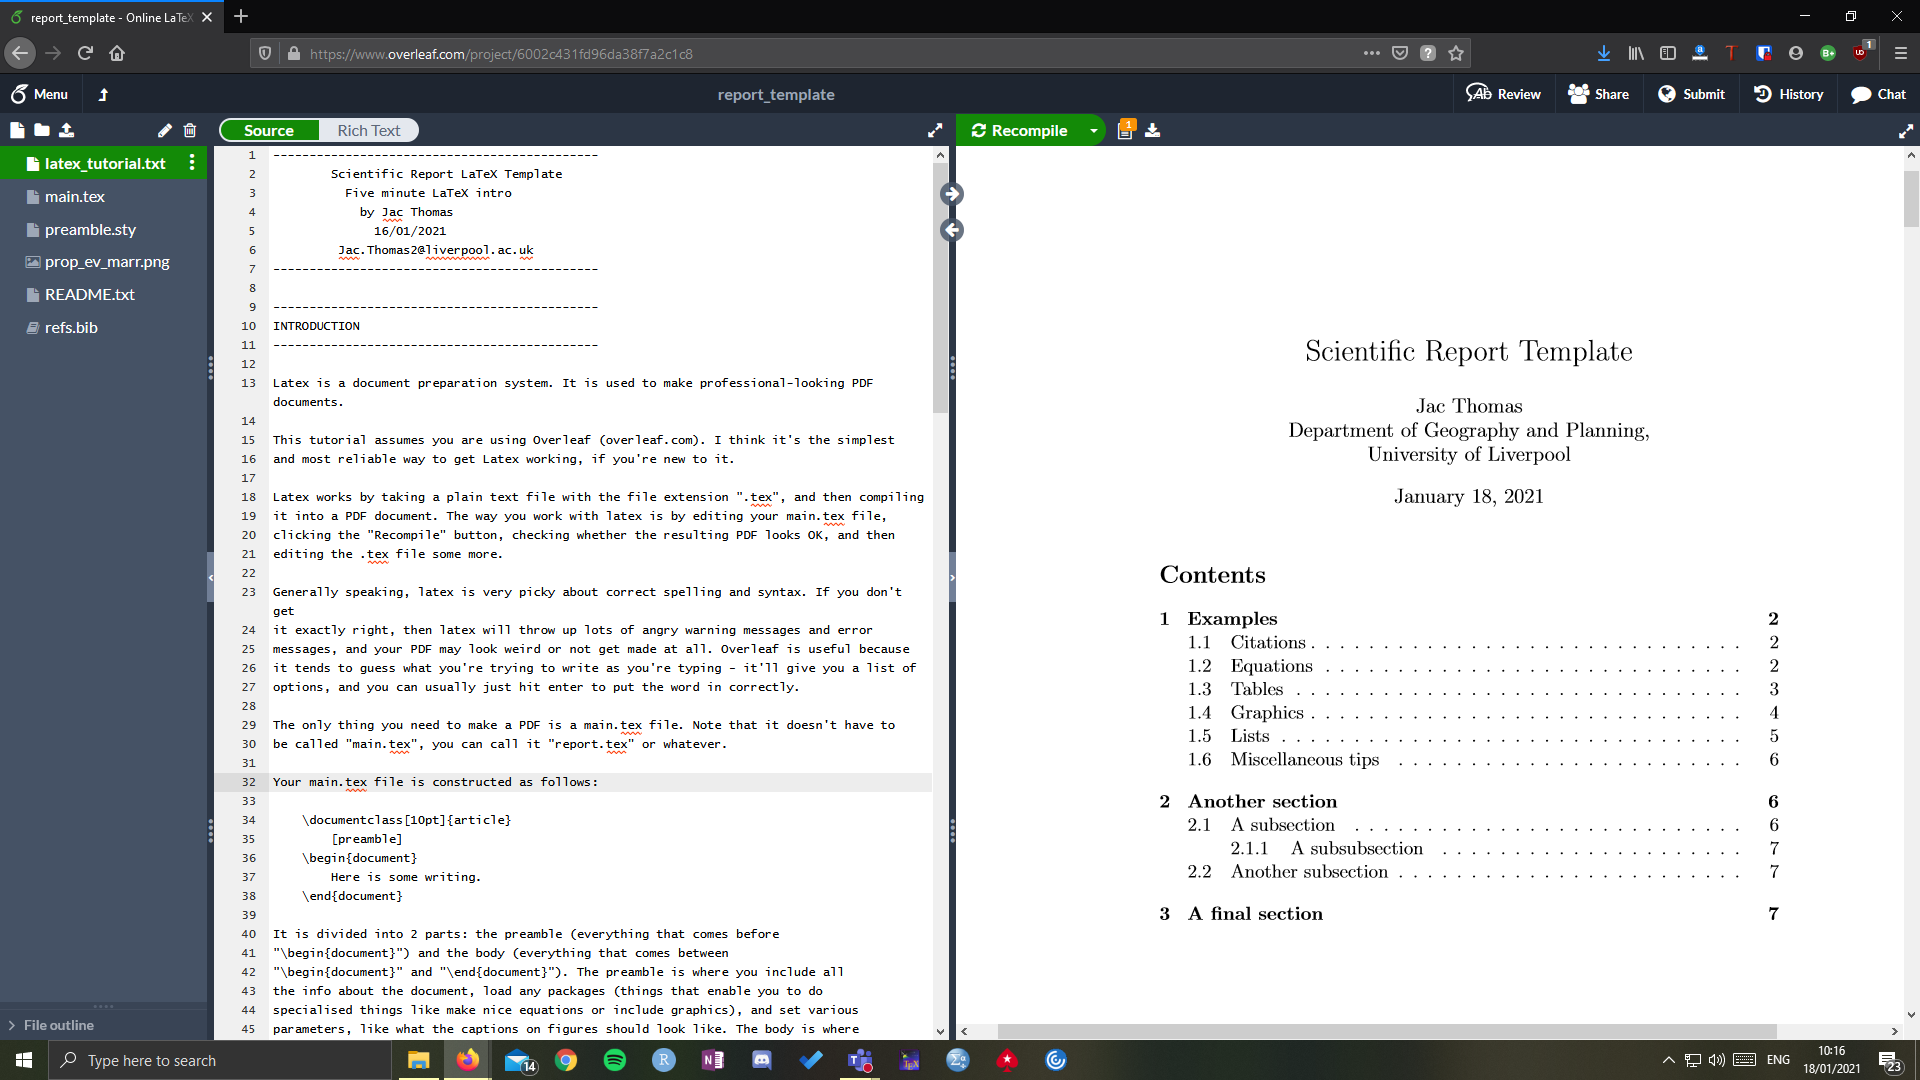
\includegraphics[scale=0.2]{screenshot.png}
    \caption{This document in Overleaf.}
    \label{fig:screenshot}
\end{figure}

\subsection{Lists}

You can start a numbered list like this.

\begin{enumerate}
    \item This is my first item.
    \item And this is the second.
\end{enumerate}

You can create a set of bullet points in a similar way.

\begin{itemize}
    \item This
    \item Is
    \item My
    \item Plan of action
\end{itemize}

\subsection{Miscellaneous tips}

This is how you make a footnote.\footnote{Here is the footnote.} This is how you write ``latex'' in a fancy way: \LaTeX.

\subsection{Further reading}

For an introduction to \LaTeX that takes more than 10 minutes, check out ``The Not So Short Introduction to \LaTeXe: Or \LaTeXe in 139 Minutes'' (\url{http://tug.ctan.org/info/lshort/english/lshort.pdf}). This is near enough the authoritative introduction to \LaTeX, and my knowledge doesn't really extend beyond its material. Apart from that, I just use the Overleaf documentation and Stack Exchange.

\section{Another section}

When she reached the first hills of the Italic Mountains, she had a last view back on the skyline of her hometown Bookmarksgrove, the headline of Alphabet Village and the subline of her own road, the Line Lane. Pityful a rethoric question ran over her cheek, then she continued her way. On her way she met a copy. The copy warned the Little Blind Text, that where it came from it would have been rewritten a thousand times and everything that was left from its origin would be the word "and" and the Little Blind Text should turn around and return to its own, safe country.

But nothing the copy said could convince her and so it didn’t take long until a few insidious Copy Writers ambushed her, made her drunk with Longe and Parole and dragged her into their agency, where they abused her for their projects again and again. And if she hasn’t been rewritten, then they are still using her. Far far away, behind the word mountains, far from the countries Vokalia and Consonantia, there live the blind texts. Separated they live in Bookmarksgrove right at the coast of the Semantics, a large language ocean. A small river named Duden flows by their place and supplies it with the necessary regelialia.

\subsection{A subsection}

Far far away, behind the word mountains, far from the countries Vokalia and Consonantia, there live the blind texts. Separated they live in Bookmarksgrove right at the coast of the Semantics, a large language ocean. A small river named Duden flows by their place and supplies it with the necessary regelialia. It is a paradisematic country, in which roasted parts of sentences fly into your mouth.

Even the all-powerful Pointing has no control about the blind texts it is an almost unorthographic life One day however a small line of blind text by the name of Lorem Ipsum decided to leave for the far World of Grammar. The Big Oxmox advised her not to do so, because there were thousands of bad Commas, wild Question Marks and devious Semikoli, but the Little Blind Text didn’t listen. She packed her seven versalia, put her initial into the belt and made herself on the way.

\subsubsection{A subsubsection}

But nothing the copy said could convince her and so it didn’t take long until a few insidious Copy Writers ambushed her, made her drunk with Longe and Parole and dragged her into their agency, where they abused her for their projects again and again. And if she hasn’t been rewritten, then they are still using her. Far far away, behind the word mountains, far from the countries Vokalia and Consonantia, there live the blind texts. Separated they live in Bookmarksgrove right at the coast of the Semantics, a large language ocean. A small river named Duden flows by their place and supplies it with the necessary regelialia.

\subsection{Another subsection}

When she reached the first hills of the Italic Mountains, she had a last view back on the skyline of her hometown Bookmarksgrove, the headline of Alphabet Village and the subline of her own road, the Line Lane. Pityful a rethoric question ran over her cheek, then she continued her way. On her way she met a copy. The copy warned the Little Blind Text, that where it came from it would have been rewritten a thousand times and everything that was left from its origin would be the word "and" and the Little Blind Text should turn around and return to its own, safe country.

\section{A final section}

But nothing the copy said could convince her and so it didn’t take long until a few insidious Copy Writers ambushed her, made her drunk with Longe and Parole and dragged her into their agency, where they abused her for their projects again and again. And if she hasn’t been rewritten, then they are still using her. Far far away, behind the word mountains, far from the countries Vokalia and Consonantia, there live the blind texts. Separated they live in Bookmarksgrove right at the coast of the Semantics, a large language ocean. A small river named Duden flows by their place and supplies it with the necessary regelialia.

\newpage

\printbibliography

\end{document}
